\chapter{Introduzione ad Apache Solr}

Come visto nel capitolo precedente, realizzare un sistema di reperimento delle informazioni richiede che vangano affrontati numerosi problemi, talvolta anche molto complessi. Per questo motivo, qualora vi sia la necessità di progettare e sviluppare un proprio motore di ricerca, è possibile contare su alcune soluzioni già esistenti. Fra le più conosciute vi è \textbf{Apache Lucene}\footnote{\url{http://lucene.apache.org/}} una libreria open source scritta in Java che offre funzioni di ricerca \textit{full text}. Lucene si occupa personalmente della gestione fisica degli indici inversi e mette a disposizione apposite funzionalità per schematizzare le informazioni a disposizione, sulle quali condurre un’ampia gamma di interrogazioni.

Nonostante esistano porting della libreria Java in numerosi altri linguaggi di programmazione, può rivelarsi tediante sviluppare motori di ricerca complessi con il solo utilizzo di Lucene. Per questa ragione nasce \textbf{Apache Solr}\footnote{\url{https://lucene.apache.org/solr/}}, una piattaforma di \textbf{\textit{enterprise search}} costruita su Lucene stesso che offre funzionalità di alto livello, il cui utilizzo si rivela adatto all’interno di sistemi dalle dimensioni importanti con ampie esigenze informative. Solr si occupa di organizzare e gestire alcuni aspetti che non sono di facile gestione con Lucene e permette di configurare il sistema in maniera più rapida ed efficace.




\section{Enterprise Search}

Il termine \textit{enterprise search} è utilizzato per descrivere finalità di ricerca progettate per il reperimento delle informazioni all’interno di contesti specifici e di natura aziendale. Si contrappone al concetto di \textit{web search}, che opera con le risorse pubblicamente disponibili nel World Wide Web.

Nonostante la vera e propria funzionalità di ricerca possa di fatto essere resa disponibile anche al di fuori delle mura aziendali, la base documentale con cui ha a che fare un software di \textit{enterprise search} appartiene al dominio dell’azienda ed è frutto dell’aggregazione di molteplici sorgenti. In funzione di questa varietà delle fonti, è ricorrente la necessità di gestire documenti con significati e rappresentazioni molto differenti fra loro. L’obiettivo consiste nel fornire l’opportunità all’utente di effettuare ricerche efficaci ed intuitive sulla base documentale, senza che egli si renda conto dell’eterogeneità delle informazioni a propria disposizione.

Un software di \textit{enterprise search} elabora e mette a disposizione per la ricerca dati che prevengono non solo da uno o più database, quindi ben strutturati, ma anche memorizzati e scambiati tramite qualsiasi altro mezzo aziendale che fornisca l’accesso a molteplici tipi di documenti, comunicazioni, file di log, calendari, mappe, etc., le quali costituiscono informazioni non strutturate o semi-strutturate all’interno delle quali è difficile orientarsi se non le si elabora nella maniera adeguata.

\vspace{1em}

L’utente che deve utilizzare un software aziendale per finalità di ricerca:
\begin{itemize}
\item Conosce il dominio applicativo d’utilizzo;
\item Vuole reperire velocemente informazioni dall’enorme quantità di dati; 
\item Vuole poter ritrovare facilmente elementi di cui conosce già l’esistenza;
\item Vuole che la ricerca sia proficua ed eventualmente raffinarne i risultati;
\item Vuole che il sistema conosca il contesto applicativo e sia quindi in grado di effettuare le dovute inferenze;
\item Vuole minimizzare i propri sforzi.
\end{itemize}

\vspace{0.45em}

Tali esigenze corrispondo agli obiettivi da tenere a mente in fase di progettazione di un motore di ricerca e costituiscono i punti di riferimento che hanno accompagnato la realizzazione del mio progetto di \textit{enterprise search} e, pertanto, guidano la stesura di questa tesi. Prima di affrontare il caso di studio analizzato vorrei dedicare un capitolo ad Apache Solr, per spiegarne il funzionamento di base e comprendere quali sono le soluzioni che propone per affrontare problemi ricorrenti di Information Retrieval.




\section{Cos’è Apache Solr}

Apache Solr è una piattaforma di \textit{enterprise search} che nasce nel 2004, il cui progetto si sviluppa nel corso degli anni al fianco di Lucene, una libreria Java rilasciata sotto licenza Apache che implementa soluzioni di Information Retrieval, ed in particolare l’indicizzazione e la ricerca \textit{full text}.

\vspace{1em}
Come Lucene, anche Solr è open source, scritto in Java e può vantare un’ampia comunità di persone che lo utilizzano e contribuiscono al suo sviluppo. Nasce con lo scopo di ampliare le funzionalità di Lucene per renderlo più scalabile e versatile, ma anche più facilmente utilizzabile grazie ad interazioni ad alto livello. Utilizzare una piattaforma del calibro di Solr consente di gestire il processo di ricerca a 360 gradi, totalmente configurabile sulla base delle proprie esigenze funzionali e architetturali. 

\vspace{1em}
Ciò ne giustifica l’utilizzo rispetto ad altri sistemi che pur offrendo funzionalità di \textit{full text search}, come ad esempio alcuni DBMS\footnote{Ho personalmente effettuato un confronto fra la funzionalità di ricerca testuale di Solr e del DBMS NoSQL document-based MongoDB ed è emerso che quest’ultimo, nonostante riesca ad equiparare Solr riguardo molte opportunità di ricerca e tempi di esecuzione, si rivela carente nel momento in cui si hanno esigenze di ricerca più avanzate come ad esempio un’analisi linguistica completa di sinonimi e tesauri oppure funzionalità fortemente tipiche di enterprise search systems: estrazione del testo da un file, Highlighting, Spellcheck, MoreLikeThis, etc.}, non mettono disposizione una così ampia gamma di personalizzazioni e funzionalità.



\subsection{Architettura}

Così come alcuni DBMS NoSQL, anche Solr sfrutta una memorizzazione logica di tipo \textit{document-based}, che consiste nel considerare l’unità informativa come un \textbf{documento} composto da più \textbf{campi} e rappresentato sotto forma di JSON. Tale rappresentazione appare molto comoda e adatta alla modellazione di qualsiasi tipo di informazione, in maniera versatile e facilmente gestibile.

Solr offre ed espande tutte le funzionalità di Lucene ma è di fatto un applicativo \textbf{server}, in grado di lavorare sia in modalità \textit{stand-alone} sia come sistema distribuito in rete, prendendo in tal caso il nome di \textbf{SolrCloud}. Questa caratteristica lo rende particolarmente adatto ad applicazioni che necessitano di un’architettura ampiamente scalabile e di una forte tolleranza agli errori. Se un normale server Solr lavora con indici inversi Lucene, ognuno dei quali prende il nome di \textbf{\textit{core}}, con SolrCloud si lavora in \textit{\textbf{collection}} che costituiscono lo stesso tipo di struttura dati, ma con la possibilità di effettuare repliche e shard su molteplici istanze di Solr. Una \textbf{replica} è un’intera copia degli indici, che vengono duplicati su diversi server; per \textbf{shard} si intende invece la possibilità di suddividere un unico indice su molteplici server per distribuire il carico di lavoro. Le due tecniche di scalabilità dei dati sono utilizzabili contemporaneamente, per favorire al contempo alte prestazioni (shard) e resistenza ai guasti (replica).



\subsection{Utilizzo}

Solr è un applicativo Java da eseguire in modalità server.
Fornisce una comoda interfaccia di amministrazione accessibile tramite browser, che mette a disposizione gran parte delle principali funzionalità della piattaforma, altrimenti configurabile tramite XML e interrogabile tramite API REST, per loro natura utilizzabili da qualsiasi programma e linguaggio di programmazione in grado di inviare, ricevere ed interpretare richieste HTTP. In questo risiede sostanzialmente la portabilità di Solr rispetto a Lucene, dato che risulta facilmente configurabile ed interrogabile da qualsiasi client connesso ad internet, senza che siano necessari particolari requisiti di installazione.

Ad esempio, per chiedere a Solr di indicizzare un documento è sufficiente inviarlo al server con una richiesta POST, includendolo nel body in formato JSON/XML/CSV o come file da cui estrarre il contenuto. In alternativa è possibile affidarsi a sistemi di importazione da database relazionali o sorgenti HTTP di varia natura (RSS, e-mail repository, etc.).



\subsection{Query}

Per sottoporre una query al sistema è necessario inviare una richiesta GET, specificando i parametri di ricerca nella \textit{querystring}. Solr gode di tutte le funzionalità di Lucene, proponendone di nuove. Il risultato di una ricerca, per default, presenta come risultato i documenti reperiti in ordine di rilevanza decrescente, che in Solr prende il nome di \texttt{score} (punteggio).

\begin{figure}[H]
	\centering
	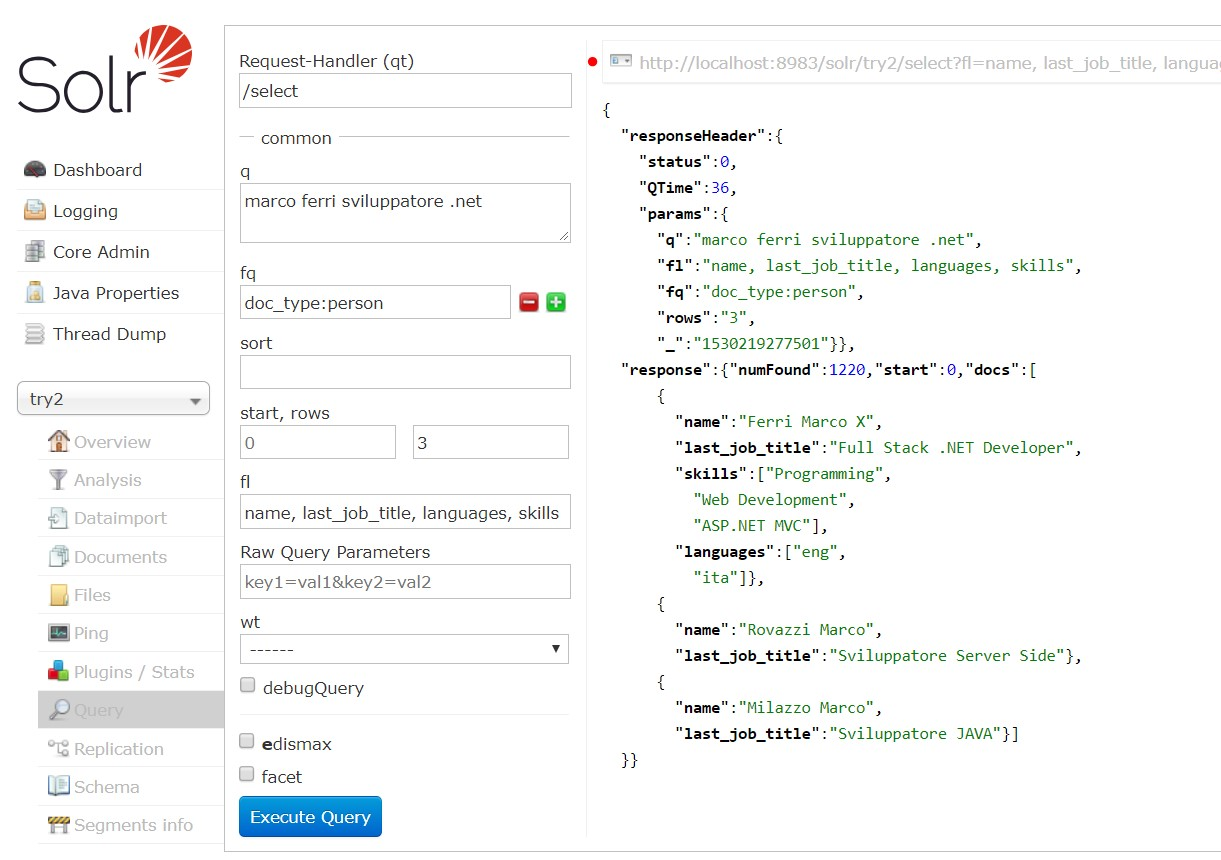
\includegraphics[scale=0.48]{../images/02_1_esempio_ricerca}
	\caption[Esempio di ricerca con Solr]{Esempio di ricerca con Solr}
	\label{fig:searchexample}
\end{figure}

\vspace{1.5em}

Nell’immagine~\ref{fig:searchexample} è possibile osservare un esempio di interrogazione, effettuata attraverso l'interfaccia web di amministrazione\footnote{\url{https://lucene.apache.org/solr/guide/7\_4/overview-of-the-solr-admin-ui.html}}, in cui vengono mostrati un limitato numero di parametri con cui è possibile effettuare la ricerca\footnote{\url{https://lucene.apache.org/solr/guide/7_4/common-query-parameters.html}}. Dallo screenshot si evince che il \textit{core} su cui si esegue la query prende il nome di \textit{try2} (lo si può notare sulla sinistra) e che i parametri di ricerca utilizzati sono i seguenti:

\begin{itemize}
\item “\texttt{q}” indica a Solr di cercare le parole \textit{marco}, \textit{ferri}, \textit{sviluppatore} e \textit{.net}. Questo parametro, se non diversamente specificato, utilizza il \textit{query parser} standard di Lucene che cerca ciascun termine in \texttt{OR} e considera per la ricerca un \textbf{campo di default} (definito nei file di configurazione). Con gli appositi parametri è possibile sfruttare altri \textit{parser}, ognuno dei quali fornisce funzionalità specifiche, e indicare diversi campi su cui effettuare la ricerca.
\item “\texttt{fq}”, letteralmente \textit{filter query}, consiste in un filtro che non influisce sullo \texttt{score} dei documenti e pertanto sul calcolo della rilevanza. In questo caso viene specificato \texttt{doc\_type}:\textit{person}, che chiede a Solr di reperire solamente i documenti con il valore \textit{person} nel campo \texttt{doc\_type}.
\item “\texttt{rows}”, pari a \texttt{3}, chiede di restituire soltanto i primi tre risultati.
\item “\texttt{fl}”, che significa \textit{field list}, specifica quali campi (o \textbf{field}) dei documenti trovati devono essere inclusi nel risultato. 
\end{itemize}

\noindent
La query dell'esempio è il risultato di una richiesta al seguente url \newline
{\small\url{http://localhost:8983/solr/try2/select? fl=name,\%20last\_job\_title,languages,skills\&fq=doc\_type:person\&q=marco\%20ferri\%20sviluppatore\%20.net\&rows=3}} %\newline
e produce una risposta che vede \texttt{1220} risultati trovati (\texttt{numFounds}), ordinati per rilevanza decrescente, di cui vengono mostrati in formato JSON solamente i primi tre. È importante notare che non tutti i documenti trovati contengono la totalità delle parole cercate, vista la ricerca in \texttt{OR}, ma che il primo risultato le contiene tutte, seppur il termine \textit{sviluppatore} appaia in realtà con il suo sinonimo \textit{developer}.

\vspace{2em}

Fra le altre funzionalità disponibili in fase di interrogazione vi è la possibilità di effettuare dei \textbf{\textit{boosting}}, cioè di specificare che alcuni campi o termini della query vengano considerati più o meno importanti di altri per il calcolo della rilevanza, influenzando così l’ordine di presentazione dei risultati.

Un ulteriore strumento molto utile consiste nelle \textbf{ricerche geo-spaziali}: Solr è in grado, dato un punto geografico rappresentato da latitudine e longitudine, di reperire tutti i documenti che specificano una posizione geografica (espressa anch’essa in coordinate) entro una certa distanza dal punto di partenza.



\subsection{Funzionalità}

Oltre alle classiche funzionalità di ricerca \textit{full text}, Solr ne mette a disposizione molte altre pensate per applicazioni che fanno della ricerca il proprio punto cardine. Alcune di queste vengono ora presentate in maniera molto rapida e verranno approfondite meglio nel capitolo successivo, per comprendere in che modo siano state utilizzate all’interno del motore di ricerca da me progettato e realizzato.



\pagebreak
\subsubsection{Faceting e Grouping}

\begin{wrapfigure}[18]{r}{5cm}
  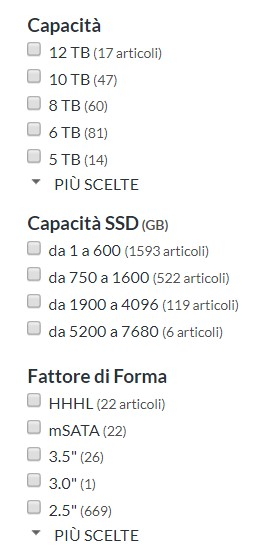
\includegraphics[scale=0.58]{../images/02_2_faceting}
  \caption[Esempio di faceting]{Faceting}
  \label{fig:facetingexample}
\end{wrapfigure} 

Il \textit{faceting}, difficilmente traducibile in italiano se non con il termine “ricerca sfaccettata”, è un tipo di ricerca ampiamente conosciuta ed utilizzata sui principali portali di compra-vendita e non solo.
Consiste in un insieme di \textbf{filtri su specifici campi}, che dispongono solitamente di una sorta di “\textbf{conteggio}” atto ad indicare quanti dei documenti risultanti dalla query soddisfano uno specifico valore del filtro. Nell’immagine~\ref{fig:facetingexample}, un esempio - riguardante la ricerca di un hard disk - preso da un noto sito di e-commerce potrà sicuramente chiarire qualsiasi dubbio circa il significato del termine \textit{faceting}.

\vspace{1em} 
Questa funzionalità è, insieme al \textbf{raggruppamento per campo}, una delle principali caratteristiche di un sistema di \textit{enterprise search}, perché estremamente utile all’utente per raffinare i risultati della ricerca in essere o semplicemente visualizzare in maniera rapida quali sono le “categorie” cui i risultati reperiti appartengono.

\subsubsection{Highlighting}

L’\textit{highlighting} è la tecnica che consente di \textbf{mettere in evidenza i termini} cercati (e trovati) all’interno di un documento, solitamente mettendoli graficamente in risalto. È tipico degli snippet di Google ed è uno strumento utilissimo per gli utenti, specie per quando si sta effettuando una ricerca all’interno di testi molto lunghi o non si riesce a comprendere il motivo per cui un determinato documento sia stato giudicato come rilevante da parte del sistema.


\subsubsection{Spellcheck \& Suggester}

Chiunque si sarà imbattuto nella scritta \textit{“Forse cercavi...”}, tipica dei più comuni motori di ricerca online. In Solr questa funzione prende il nome di \textit{spellcheck} e può essere utile per \textbf{correggere} (anche in maniera automatica) le parole specificate dall’utente nella query. In combinazione con il \textit{suggester}, che fornisce \textbf{autocompletamento} delle query, ha lo scopo di ridurre ricerche fallimentari causate da errori di battitura.


\subsubsection{MoreLikeThis}

Ancora una volta scenario tipico dei motori di ricerca sul Web, che si tratti di siti di compravendita o ricerca per immagini, questa funzionalità permette all’utente di dare in pasto a Solr un certo documento affinché il sistema si occupi di cercare nell'indice tutti i \textbf{documenti simili} ad esso. Funzione molto usata per fini commerciali.




\section{Modellazione dei dati con Solr}

\begin{wrapfigure}[12]{r}{5.2cm}
  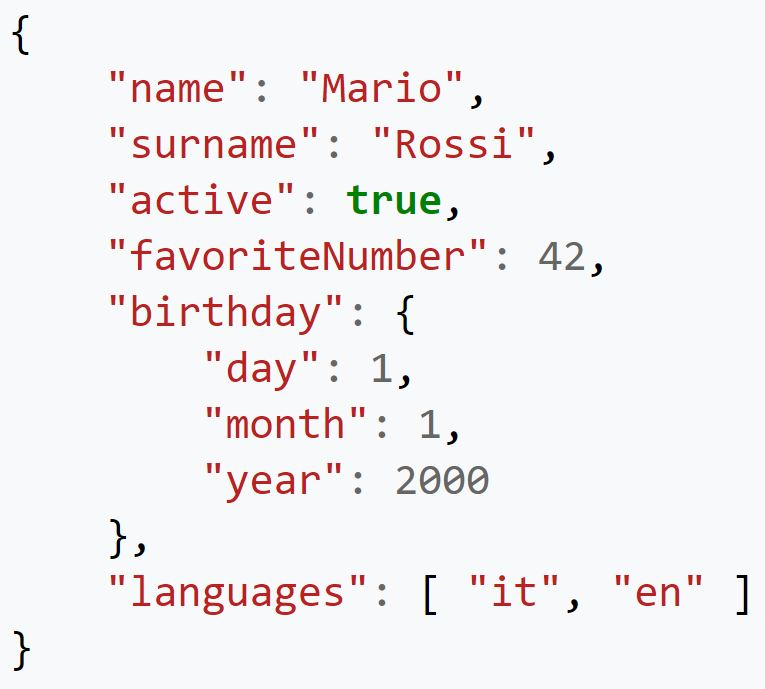
\includegraphics[scale=0.32]{../images/02_3_json}
  \caption[Esempio di JSON]{JSON}
  \label{fig:jsonexample}
\end{wrapfigure} 

Come precedentemente accennato, l’entità base che costituisce informazione in Solr è il documento, rappresentato sotto forma di JSON. Chiunque sia familiare a questo tipo di formato comprende istantaneamente l’importanza che ha assunto nell’ultimo ventennio per lo scambio di informazioni online e più recentemente anche come modello di memorizzazione nei più recenti DBMS. Un JSON è perfettamente adatto a rappresentare il \textit{record} di un database relazionale o l’\textit{oggetto} di un linguaggio di programmazione \textit{object-oriented} e data la sua versatilità si rivela adatto a modellare le informazioni eterogenee con cui una piattaforma di\textit{ enterprise search} ha costantemente a che fare. 



\subsection{Schema e tipizzazione}

Essendo la rappresentazione JSON costituita da un insieme di proprietà \texttt{nome:"valore"} (figura~\ref{fig:jsonexample}), è chiaro che tali proprietà devono essere opportunamente memorizzate da Solr all’interno degli indici inversi, che per ereditarietà da Lucene sono in grado di suddividere le informazioni di ogni documento in specifici \textbf{campi} (o \textit{field}).

È possibile, per ogni \textit{core} di Solr, definire uno \textbf{schema} che descrive la struttura dei documenti all’interno dell’indice, oppure affidarsi ad un approccio \textbf{\textit{schemaless}}. Nel primo caso, il server sarà in grado di indicizzare esclusivamente documenti che contengono i soli campi dichiarati nello schema (o alcuni di essi) e rifiuterà tutto ciò che non è conforme. Al contrario, se si sceglierà di sfruttare la tecnica \textit{schemaless}, qualsiasi tipo di documento potrà essere \textit{postato}, delegando a Solr la creazione di campi finora sconosciuti. Questo secondo approccio è molto utile se non si conosce la composizione dei documenti che faranno parte dell’indice o se lo schema è frequentemente soggetto ad aggiornamenti, ma è generalmente sconsigliato per software in ambiente di produzione.

\vspace{1em}

Ciascun campo che appartiene ad un documento Solr è \textbf{fortemente tipizzato}, che esso sia esplicitamente dichiarato nello schema o inferito automaticamente dal sistema quando ne crea di nuovi. Tutti i tipi di campo descritti nello schema sono mappati con opportune classi Java che ne definiscono il comportamento di base. Poi, per ogni tipo, è possibile specificare una \textbf{catena di analisi testuale} personalizzata, che indica quali devono essere le operazioni da eseguire sul contenuto dei campi di un certo tipo, prima che il testo dei documenti (e più precisamente i termini) vengano indicizzati da Solr.

La tipizzazione dei campi consente di definire comportamenti altamente specifici per ognuno di essi e permette all’amministratore Solr di scegliere quale dev’essere la granularità di ricerca per ciascun tipo definito nello schema. Per esempio, può capitare che alcune informazioni debbano essere trattate come un unico termine seppur appaiono intervallate da caratteri separatori (e.g., IBAN bancari, codici fiscali, etc.), o che alcuni campi necessitino di analisi linguistiche personalizzate.

\vspace{1em}

Con Solr l’analisi testuale dei processi di indicizzazione e interrogazione è ben distinta, ma è essenziale che i due trattamenti siano compatibili affinché l’algoritmo di \textit{matching} sia in grado di confrontare i termini dei documenti e quelli della query in maniera consistente.



\subsection{Content Extraction Library}
\label{sec:solrcell}

Si è precedentemente accennato all’eterogeneità delle fonti che costituiscono la base documentale di un sistema di reperimento delle informazioni, in particolare per quanto riguarda software di enterprise search. 

Se le tabelle di un database sono facilmente esportabili in JSON, non è altrettanto vero per quanto riguarda i file memorizzati sul disco fisso. Come è possibile immaginare, non tutti i file sono adatti ad un’estrazione diretta del testo, perché la maggior parte di essi sono in un formato binario (e.g., doc, pdf, xls, ppt, etc.) oppure contengono dati “sporchi”, come nel caso dei file XML, HTML o delle email, di cui solitamente non si vuole indicizzare direttamente il testo che compone tag o intestazioni. Solr ci viene in aiuto, mettendo a disposizione la propria \textit{Content Extraction Library} (Solr CELL), che sfrutta il progetto \textbf{Apache Tika}\footnote{\url{https://tika.apache.org/}} per estrarre testo e metadati da un qualsiasi file.

\vspace{1em}

Il contenuto testuale estratto da un file sarà assegnato ad un campo scelto arbitrariamente, soggetto alla catena di analisi testuale prevista per quel campo. L’analisi dei file rappresenta una delle operazioni più stressanti per il sistema, per via dell’enorme quantità di \textit{token} solitamente estratti dal file stesso, che dovranno essere singolarmente analizzati affinché vadano a costituire i termini indice.

Proprio a causa di questa numerosità, è opportuno decidere in fase di progettazione se è opportuno, oltre che indicizzare, anche “memorizzare” il contenuto estratto dai file. Un campo indicizzato (\texttt{indexed}) ma non memorizzato (\texttt{not stored}) è disponibile per la ricerca e il meccanismo di \textit{matching} fra query e documenti ne terrà conto, ma non verrà mostrato fra i risultati della ricerca stessa. In altre parole, se un certo file contiene un termine della query, il documento che rappresenta tale file verrà mostrato fra i risultati della ricerca, ma privo del campo \texttt{not stored} su cui è stata realmente effettuata la ricerca. Scegliere di non memorizzare il contenuto estratto da un file può risparmiare moltissimo spazio sulla memoria di massa del server Solr, ma introduce alcune limitazioni che si vedranno più avanti.




\pagebreak
\section{Algoritmo di matching basato su Okapi BM25}

A conclusione del capitolo, ci si ricollega ai modelli matematici che costituiscono un sistema di reperimento delle informazioni cui si faceva riferimento nel capitolo~\ref{sec:mathmodels}, per fornire una breve spiegazione di quello che è l’attuale\footnote{Nel momento in cui scrivo questa tesi, e quindi con riferimento alla versione 7.4 di Solr} algoritmo di \textit{matching} di default utilizzato da parte di Solr.

\vspace{1em}
Il suo nome è Okapi BM25 e vede la luce nel lontano 1994. \newline
Si tratta di un modello di tipo \textbf{probabilistico}, che considera il concetto di rilevanza come la probabilità che un certo documento possa o meno essere considerato rilevante da parte dell’utente. Nello specifico, Okapi BM25 basa il proprio funzionamento su un’evoluzione del modello \textit{TF*IDF (term frequency * inverse document frequency)}, funzione di pesatura dei termini presentata nella sezione~\ref{sec:termsweight}. 

\vspace{1em}

All’algoritmo di base vengono apportate diverse modifiche e miglioramenti, il cui elemento chiave è la nuova modalità di calcolo della \textit{inverse document frequency}, che ora costituisce la componente probabilistica di BM25 . Anche la trattazione della \textit{term frequency} e della \textit{lunghezza del documento} sono state riviste, affinché la prima si riveli meno incisiva nel calcolo della rilevanza mentre la seconda possa essere soggetta ad un maggiore controllo. Approfondimenti ulteriori vanno oltre lo scopo di questa tesi e per maggiori dettagli si rimanda ad un articolo in bibliografia~\cite{bm25_osc} che spiega questi concetti in maniera molto chiara ed evidenzia che, seppur BM25 sia un modello con molte potenzialità, non è detto si riveli adatto a qualsiasi situazione.

% INSERIRE FOMULA
\[score(D,Q) = \sum\limits_{i=1}^n IDF(q_{i}) \times \frac{f(q_{i}, D) \times (k_{1} + 1)}{f(q_{i}, D) + k_{1} \times (1 - b + b \times \frac{|D|}{avgdl})}\]

Il risultato consiste di questa formula abbastanza complessa - all’interno della quale compaiono alcuni parametri di normalizzazione - che va sostanzialmente a considerare l’insieme delle caratteristiche presentate già nel primo capitolo di questa tesi. Ciò va a dimostrazione del fatto che un buon algoritmo di \textit{matching}, per quanto complesso possa rivelarsi, consiste principalmente nel trovare la giusta combinazione dei concetti di base dell’Information Retrieval precedentemente presentati.





















